The following class diagramm includes all classes/interfaces of the
data subpackage. This package fulfills the task of reading {*}.etis
files and to translate the contained information into corresponding
data structures:

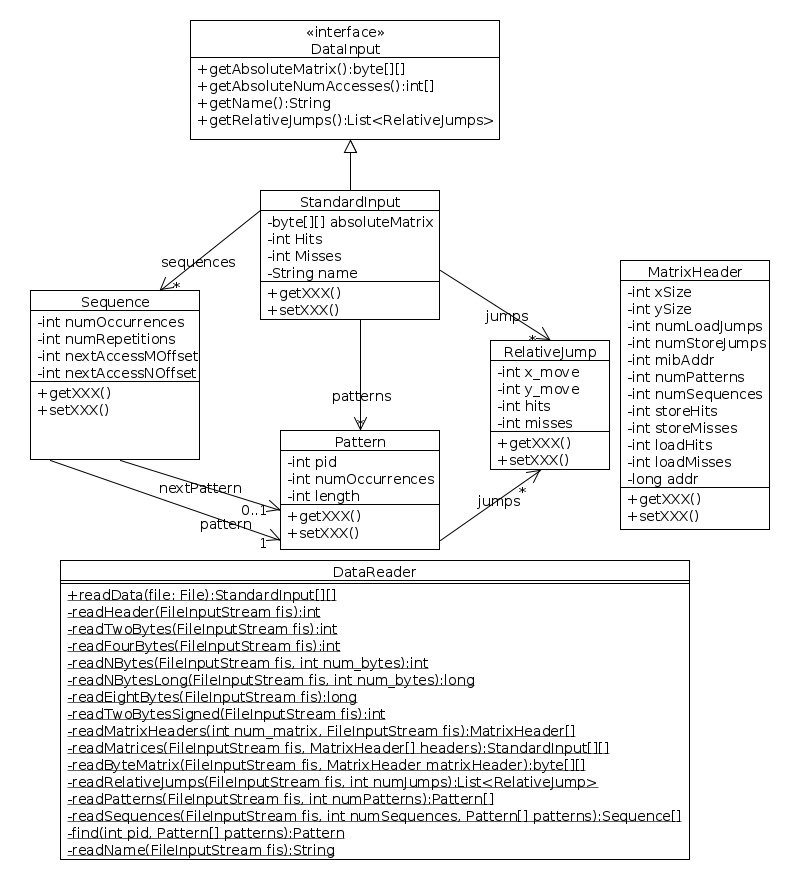
\includegraphics[scale=0.55]{gui/DataClassDiagram.png}

\texttt{getXXX()/setXXX()} is used here as a shorthand to indicate
that the classes have corresponding getters/setters for every private
attribute. The \texttt{DataReader} class exports the central method
of the package, namley \texttt{readData}. It takes a \texttt{File}
object as an argument and tries to read it as a file in the {*}.etis
format. It returns a length two array of \texttt{StandardInput} objects
for every matrix that is contained in the file. In one of those arrays
the first object always contains all the information about load type
accesses and the second one contains all the store type access information.
As patterns and sequences do not distinguish between load and store
this information will only be contained in the \texttt{StandardInput}
object for load. In order to fulfill the job of reading {*}.etis files,
the \texttt{DataReader} class defines a few static helper methods:
First of all there are some methods that can read different numbers
of consecutive bytes in the little endian format from a \texttt{FileInputStream}
object into an integer/long (all of them but \texttt{readTwoBytesSigned}
work on unsigned numbers); second we have methods that cover the read
process for different parts of the data format - taken together with
the data format specification their names should be quite self explanatory.

The following code excerpt shows how those helper functions play together
to read a {*}.etis file:

\lstinputlisting[language=Java]{gui/ReadProcOverview.java}

The information contained in a \texttt{StandardInput} object is the
name of the matrix, the number of hits/misses on the matrix (either
for loads or stores) and the absolute access matrix (again either
for loads or stores). It also links to a number of \texttt{Sequence}
objects, a number of \texttt{Pattern} objects and a number of \texttt{RelativeJumps}
objects. Those should be quite self explanatory as they simply contain
all the information as specified in the data format specification.
Also the pattern that is repeated in a sequence and a possible next
pattern of a sequence are directly referenced in the fields \texttt{pattern}
and \texttt{nextPattern} of the \texttt{Sequence} object.

The \texttt{MatrixHeader} class is only there for intermediate use
in the read process. At last the \texttt{DataInput} interface has
become quite obsolete in the software development process, but is
still kept alive for compability with older code parts in the GUI.
